\begin{spacing}{1}

    \chapter*{Abstract}

\end{spacing}

\begin{wrapfigure}{r}{0.3\textwidth}

    \begin{center}

        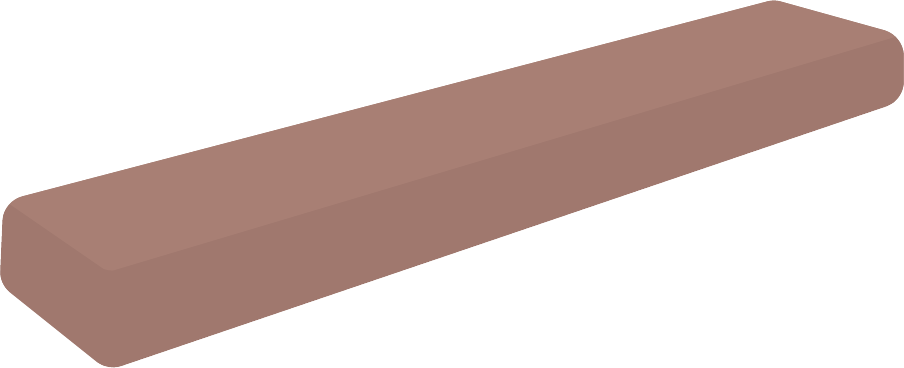
\includegraphics[width=0.2\textwidth]{pics/abstract_picture_1}

    \end{center}

\end{wrapfigure}

Beam VR is a project which aims to give an immersive experience of heights.
It consists of a scene on top of a building with plank protrudes of the building.
To increase the immersion of the reality we use virtual reality combined with the physical reality.
With a filling environment including realistic car behavior, high skyscrapers, immersive sky and classic new york city sounds we optimize the immersion of the reality.
Furthermore it is possible to choose between 3 maps, including Night, Day and Apocalypse.

\newpage

\begin{spacing}{1}

    \chapter*{Zusammenfassung}

\end{spacing}

\begin{wrapfigure}{r}{0.3\textwidth}

    \begin{center}

        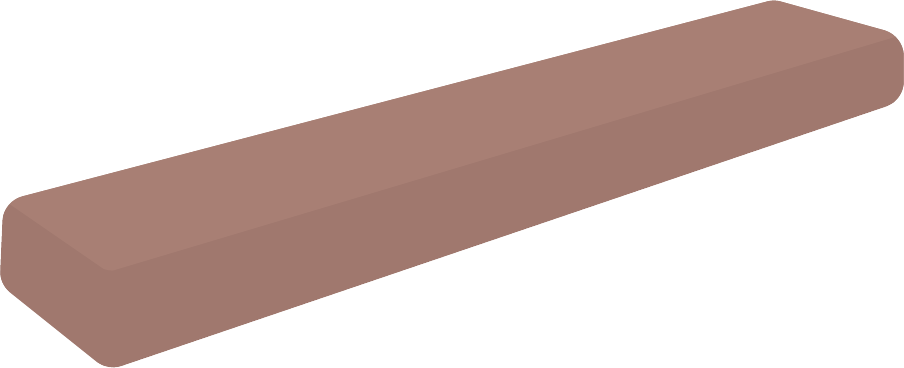
\includegraphics[width=0.2\textwidth]{pics/abstract_picture_1}

    \end{center}

\end{wrapfigure}

Beam VR ist ein Projekt, das darauf abzielt, ein immersives Höhenerlebnis zu vermitteln.
Es besteht aus einer Szene auf einem Gebäude, wobei ein Balken aus dem Gebäude herausragt.
Um die Immersion in die Realität zu erhöhen, verwenden wir die virtuelle Realität in Kombination mit der physischen Realität.
Mit einer füllenden Umgebung mit realistischem Autoverhalten, hohen Wolkenkratzern, immersivem Himmel und klassischen New-York-City-Sounds optimieren wir die Immersion.
Außerdem kann zwischen 3 Karten gewählt werden, darunter Night, Day und Apocalypse.
